%----------------------------------------------------------------------------------------

\documentclass[a4paper,10pt]{article} % Uses article class in A4 format

%----------------------------------------------------------------------------------------
%	FORMATTING
%----------------------------------------------------------------------------------------

\setlength{\parskip}{0pt}
\setlength{\parindent}{0pt}
\setlength{\voffset}{-15pt}

%----------------------------------------------------------------------------------------
%	PACKAGES AND OTHER DOCUMENT CONFIGURATIONS
%----------------------------------------------------------------------------------------

\usepackage[a4paper, margin=2.5cm]{geometry} % Sets margin to 2.5cm for A4 Paper
\usepackage[onehalfspacing]{setspace} % Sets Spacing to 1.5

\usepackage[T1]{fontenc} % Use European encoding
\usepackage[utf8]{inputenc} % Use UTF-8 encoding
\usepackage{charter} % Use the Charter font
\usepackage{microtype} % Slightly tweak font spacing for aesthetics

\usepackage[english]{babel} % Language hyphenation and typographical rules

\usepackage{amsthm, amsmath, amssymb} % Mathematical typesetting
\usepackage{marvosym, wasysym} % More symbols
\usepackage{float} % Improved interface for floating objects
\usepackage[final, colorlinks = true, 
            linkcolor = black, 
            citecolor = black,
            urlcolor = black]{hyperref} % For hyperlinks in the PDF
\usepackage{graphicx, multicol} % Enhanced support for graphics
\usepackage{xcolor} % Driver-independent color extensions
\usepackage{rotating} % Rotation tools
\usepackage{listings, style/lstlisting} % Environment for non-formatted code, !uses style file!
\usepackage{pseudocode} % Environment for specifying algorithms in a natural way
\usepackage{style/avm} % Environment for f-structures, !uses style file!
\usepackage{booktabs} % Enhances quality of tables

\usepackage{tikz-qtree} % Easy tree drawing tool
\tikzset{every tree node/.style={align=center,anchor=north},
         level distance=2cm} % Configuration for q-trees
\usepackage{style/btree} % Configuration for b-trees and b+-trees, !uses style file!

\usepackage{titlesec} % Allows customization of titles
\renewcommand\thesection{\arabic{section}.} % Arabic numerals for the sections
\titleformat{\section}{\large}{\thesection}{1em}{}
\renewcommand\thesubsection{\alph{subsection})} % Alphabetic numerals for subsections
\titleformat{\subsection}{\large}{\thesubsection}{1em}{}
\renewcommand\thesubsubsection{\roman{subsubsection}.} % Roman numbering for subsubsections
\titleformat{\subsubsection}{\large}{\thesubsubsection}{1em}{}

\usepackage[all]{nowidow} % Removes widows

\usepackage[backend=biber,style=numeric,
            sorting=nyt, natbib=true]{biblatex} % Complete reimplementation of bibliographic facilities
\addbibresource{main.bib}
\usepackage{csquotes} % Context sensitive quotation facilities

\usepackage[yyyymmdd]{datetime} % Uses YEAR-MONTH-DAY format for dates
\renewcommand{\dateseparator}{-} % Sets dateseparator to '-'

\usepackage{fancyhdr} % Headers and footers
\pagestyle{fancy} % All pages have headers and footers
\fancyhead{}\renewcommand{\headrulewidth}{0pt} % Blank out the default header
\fancyfoot[L]{\textsc{Robin Worreby}} % Custom footer text
\fancyfoot[C]{} % Custom footer text
\fancyfoot[R]{\thepage} % Custom footer text

\newcommand{\note}[1]{\marginpar{\scriptsize \textcolor{red}{#1}}} % Enables comments in red on margin
\usepackage[shortlabels]{enumitem}
\usepackage{minted}
\usemintedstyle{friendly}
\usepackage[bf]{caption}
%----------------------------------------------------------------------------------------

\begin{document}

%----------------------------------------------------------------------------------------
%	TITLE SECTION
%----------------------------------------------------------------------------------------

\title{template_assignment} % Article title
\fancyhead[C]{}
\begin{minipage}{0.295\textwidth} % Left side of title section
\raggedright
HPCSE1\\ % Your lecture or course
\footnotesize % Authors text size
%\hfill\\ % Uncomment if right minipage has more lines
Robin Worreby, 16-921-298 % Your name, your matriculation number
\medskip\hrule
\end{minipage}
\begin{minipage}{0.4\textwidth} % Center of title section
\centering 
\large % Title text size
Exercise 05\\ % Assignment title and number
\normalsize % Subtitle text size
MPI Part II % Assignment subtitle
\end{minipage}
\begin{minipage}{0.295\textwidth} % Right side of title section
\raggedleft
\today\\ % Date
\footnotesize % Email text size
%\hfill\\ % Uncomment if left minipage has more lines
rworreby@student.ethz.ch% Your email
\medskip\hrule
\end{minipage}

%----------------------------------------------------------------------------------------
%	ARTICLE CONTENTS
%----------------------------------------------------------------------------------------

\setcounter{section}{0}

\section{Parallel Scaling}

For the strong scaling we calculate the speedup with the following formula:
\begin{equation}\label{speedup}
    S = \frac{T(1)}{T(P)}
\end{equation}
We take as reference the speed of $T(P=1)$ for the problem size $N=1000$. In order to calculate the speedup of multiple nodes we therefore calculate $S_P = \frac{T(P=1, N=1000)}{T(P=P, N=1000)}$. We choose the four values to plot as $P={1, 4, 9, 16}$. The result can be seen in Figure \ref{fig:strong_scaling}.

For the weak scaling we calculate the efficiency with the following formula:
\begin{equation}
    \eta_W = \frac{T(1)}{T(P)}
\end{equation}
Note that for the $T(P)$ the workload is $P * W(1)$, where $W(1)$ is the workload of $T(1)$.
We take as reference the speed of $T(P=1)$ for the problem size $N=500$, which has a workload $W$ of $N^2 = 500^2$. In order to calculate the efficiency of multiple nodes we therefore calculate $\eta_W = \frac{T(P=1, N=500)}{T(P=P, W=P*W(1))}$. We choose the four values to plot as $P={1, 4, 9, 16}$. Calculating for example $P=4$, we have $W(P=4) = 4 * W(P=1) = 4 * 500^2 = 1000^2$.
Plugging the result into the equation before this yields the following:
\begin{equation}\label{ex_weak}
\begin{split}
        \eta_W(P=4) = \frac{T(P=1, N=500, W=500^2)}{T(P=4, N=1000 , W=4*W(1))}
                    = \frac{T(P=1, N=500, W=500^2)}{T(P=4, N=1000 , W=1000^2)}
\end{split}
\end{equation}

The result can be seen in Figure \ref{fig:weak_scaling}.

\begin{figure}[h]
  \centering
  \begin{minipage}[t]{0.45\textwidth}
    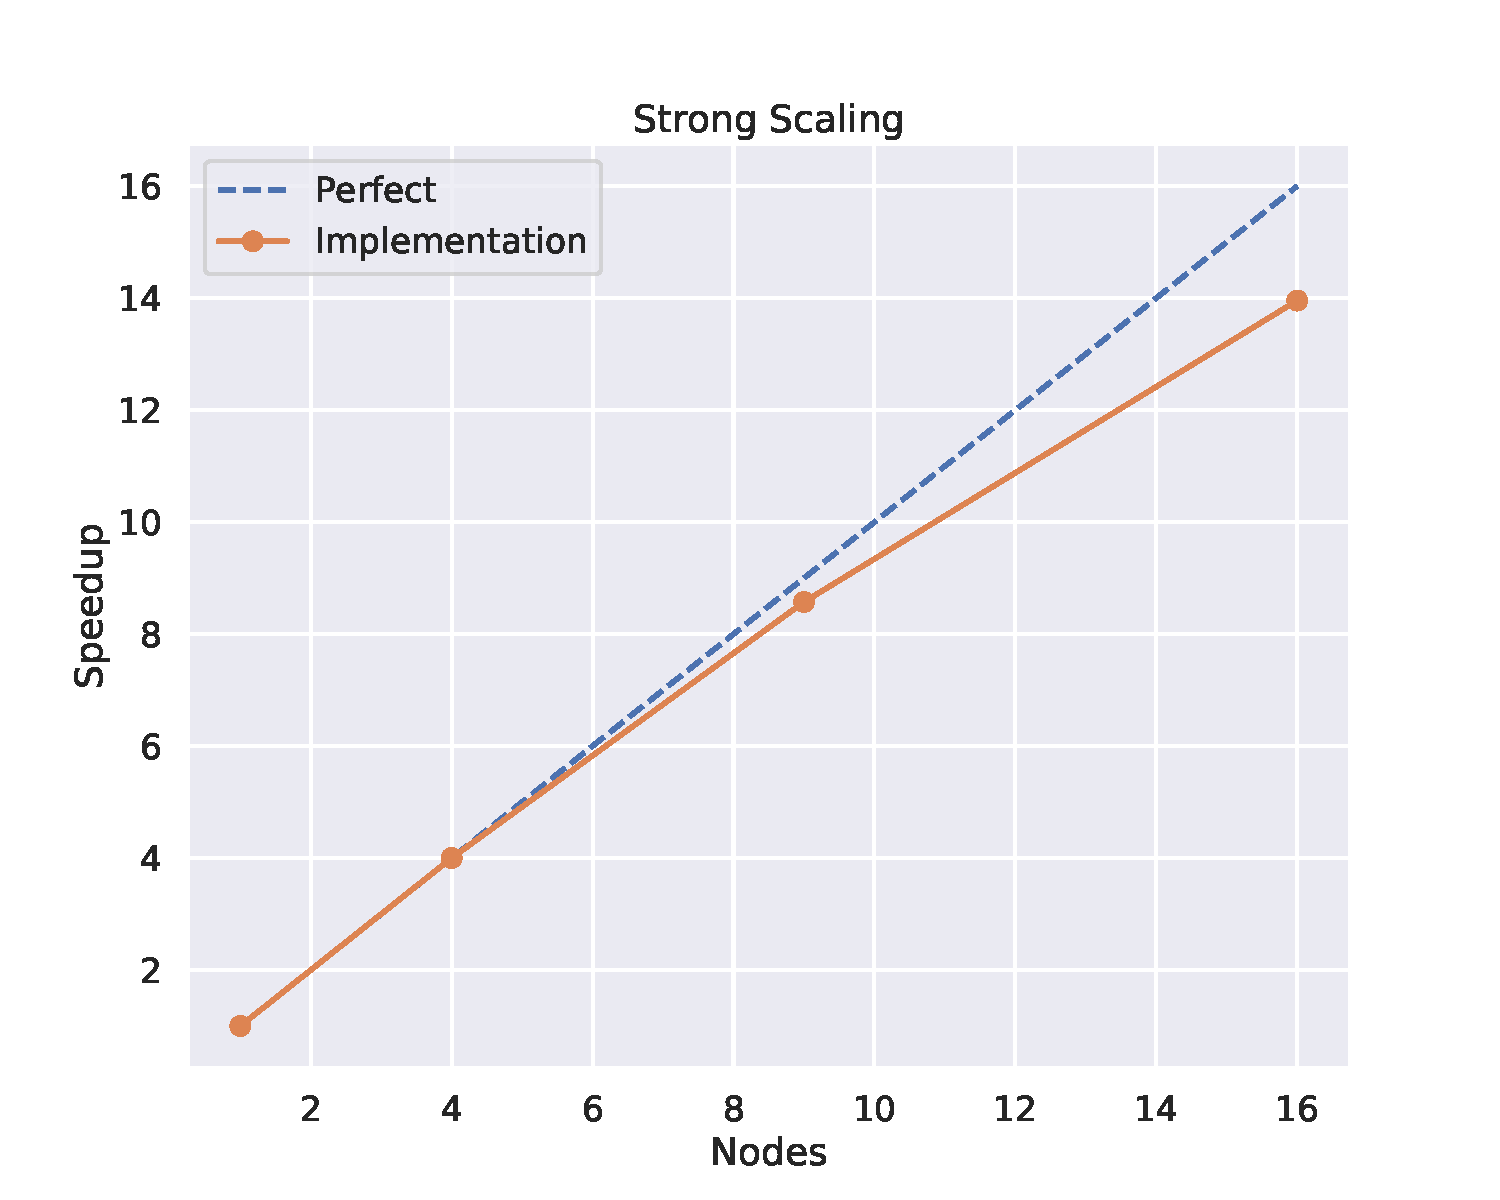
\includegraphics[width=\textwidth]{plots/strong_scaling.pdf}
    \caption{Strong scaling plot for $N=1000$ and four different $P$ values.}
    \label{fig:strong_scaling}
  \end{minipage}
  \hfill
  \begin{minipage}[t]{0.45\textwidth}
    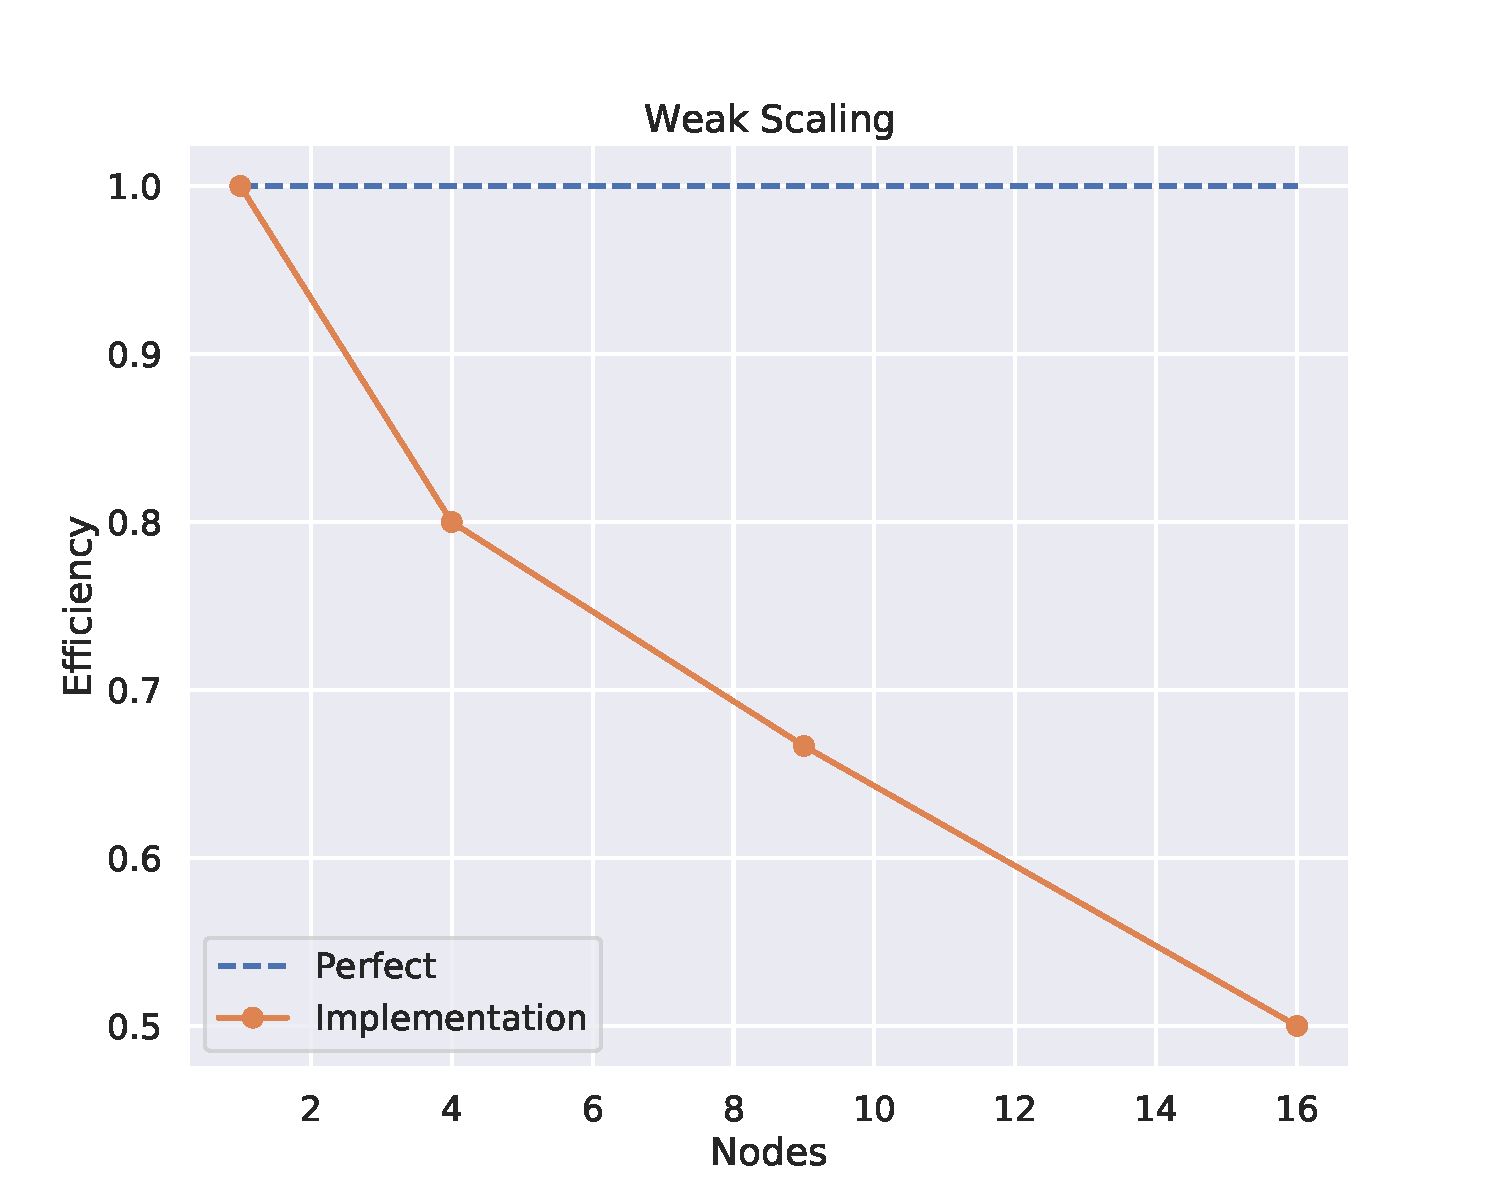
\includegraphics[width=1\textwidth]{plots/weak_scaling.pdf}
    \caption{Weak scaling plot for reference workload $P=1, N=500$.}
    \label{fig:weak_scaling}
  \end{minipage}
\end{figure}

\section{Diffusion}

\begin{figure}[H]
  \centering
  \begin{minipage}[t]{0.9\textwidth}
    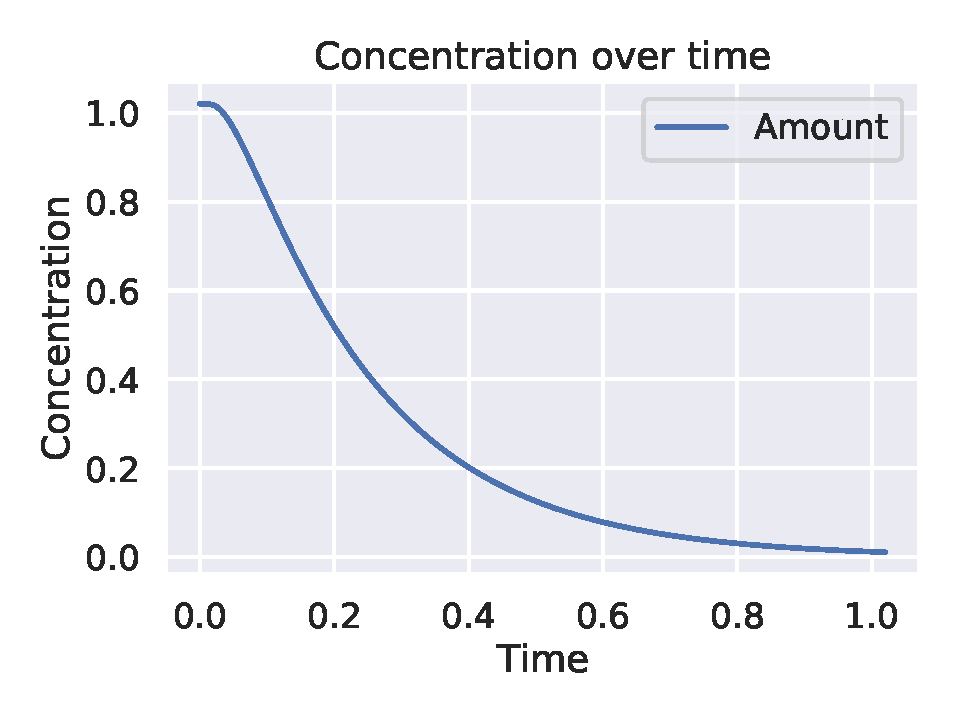
\includegraphics[width=\textwidth]{plots/concentration.pdf}
    \caption{Total concentration (substance) over time for the diffusion equation. Parameters: $D = 1, L = 2, N = 100$.}
    \label{fig:strong_scaling}
  \end{minipage}
  \hfill
  \begin{minipage}[t]{0.9\textwidth}
    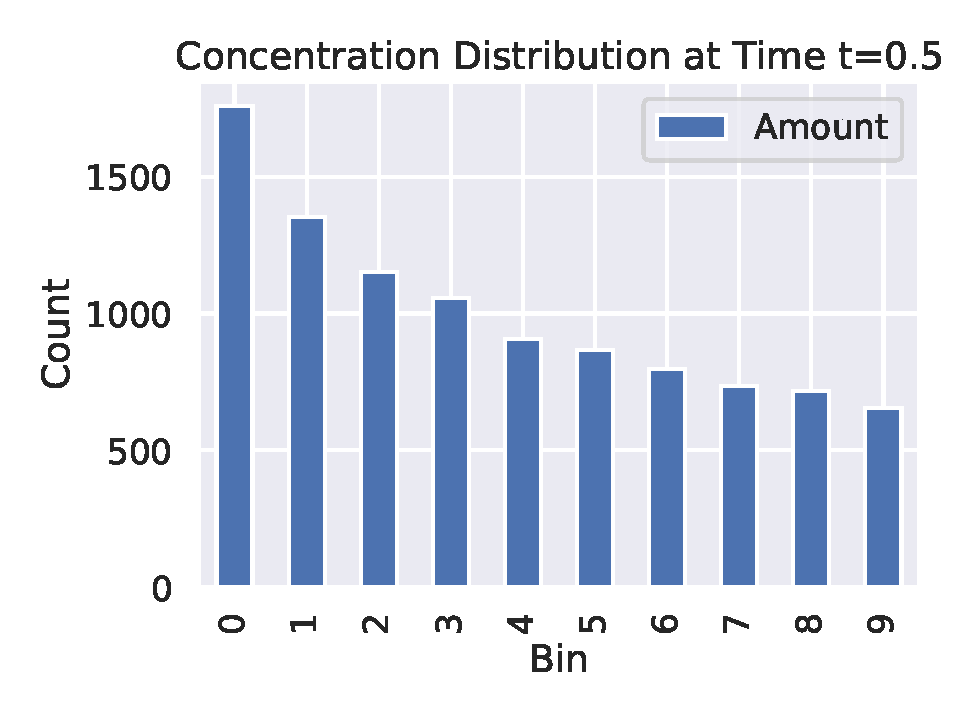
\includegraphics[width=1\textwidth]{plots/histogram.pdf}
    \caption{Distribution of concentration (substance) at time $t=0.5$ for the diffusion equation. Parameters: $D = 1, L = 2, N = 100$.}
    \label{fig:weak_scaling}
  \end{minipage}
\end{figure}

\bigskip
%----------------------------------------------------------------------------------------
%	REFERENCE LIST
%----------------------------------------------------------------------------------------

\printbibliography

%----------------------------------------------------------------------------------------

\end{document}

